\documentclass[12pt]{article}

% a template that a friend gave, it's worked well enough for me
% i have added some packages and stuff that have proved useful

\usepackage{fancyhdr}
\usepackage{tipa}
\usepackage{fontspec}
\usepackage{amsfonts}
\usepackage{enumitem}
\usepackage[margin=1in]{geometry}
\usepackage{graphicx}
\usepackage{float}
\usepackage{amsmath}
\usepackage{braket}
\usepackage{amssymb}
\usepackage{booktabs}
\usepackage{hyperref}
\usepackage{mathtools}
\usepackage{xcolor}
\usepackage{float}
\usepackage{algpseudocodex}
\usepackage{titlesec}
\usepackage{bbm}

\pagestyle{fancy}
\fancyhf{} % sets both header and footer to nothing
\lhead{Kevin Sheng}
\setmainfont{Comic Neue}
\renewcommand{\headrulewidth}{1pt}
\setlength{\headheight}{0.75in}
\setlength{\oddsidemargin}{0in}
\setlength{\evensidemargin}{0in}
\setlength{\voffset}{-.5in}
\setlength{\headsep}{10pt}
\setlength{\textwidth}{6.5in}
\setlength{\headwidth}{6.5in}
\setlength{\textheight}{8in}
\renewcommand{\headrulewidth}{0.5pt}
\renewcommand{\footrulewidth}{0.3pt}
\setlength{\textwidth}{6.5in}
\usepackage{setspace}
\usepackage{multicol}
\usepackage{float}
\setlength{\columnsep}{1cm}
\setlength\parindent{24pt}
\usepackage [english]{babel}
\usepackage [autostyle, english = american]{csquotes}
\MakeOuterQuote{"}

\setlength{\parskip}{6pt}
\setlength{\parindent}{0pt}

\titlespacing\section{0pt}{12pt plus 4pt minus 2pt}{0pt plus 2pt minus 2pt}
\titlespacing\subsection{0pt}{12pt plus 4pt minus 2pt}{0pt plus 2pt minus 2pt}
\titlespacing\subsubsection{0pt}{12pt plus 4pt minus 2pt}{0pt plus 2pt minus 2pt}

\hypersetup{colorlinks=true, urlcolor=blue}

\newcommand{\correction}[1]{\textcolor{red}{#1}}


\rhead{Math 131BH}

\makeatletter
\def\@seccntformat#1{%
  \expandafter\ifx\csname c@#1\endcsname\c@section\else
  \csname the#1\endcsname\quad
  \fi}
\makeatother

\DeclareMathOperator{\Fr}{Fr}
\newcommand{\lra}{\xLeftrightarrow}
\newcommand{\ra}{\xRightarrow}
\newcommand{\N}{\mathbb{N}}
\newcommand{\R}{\mathbb{R}}
\newcommand{\Z}{\mathbb{Z}}
\newcommand{\Q}{\mathbb{Q}}
\newcommand{\norm}[1]{\left\lVert#1\right\rVert}

\begin{document}

\section{Problem 1}

BWOC let $\left|f'(c)-\lim_{x \to c} f'(x)\right| = d > 0$.
I'll call the value of the limit $L$ for convenience.

Choose $\delta$ s.t. $x \ne c \land |x-c| < \delta \implies |f'(x)-L| < \frac{d}{2}$.

Now, for any $x \in (c, c+\delta)$ can be at most $\frac{d}{2}$ away from $L$.
However, by the intermediate value property of the derivative,
there must exist some $x$ in the interval that's $\frac{3d}{4} > \frac{d}{2}$
away from $L$, which is a contradiction. $\square$

\section{Problem 2}

\subsection{Continuous}

I'll start off assuming $f_n(x)=\frac{1}{2^n} \sin\left(3^nx\right)$
is differentiable by common sense.
With this variable we can then write $f(x)=\sum_{n=1}^{\infty} f_n(x)$.

Fix $x$ and $\epsilon > 0$.

Since $|\sin(x)| \le 1$, $|\sin(x)-\sin(y)| \le 2$ and we can choose an $N$ s.t.
\[\sum_{n=N}^{\infty} |f_n(x)-f_n(y)| \le \sum_{n=N}^{\infty} \frac{1}{2^n} \cdot 2 < \frac{\epsilon}{2}\]

Then we choose a $\delta_n$ for each $n < N$ s.t. $|x'-x| < \delta_n \implies |f_n(x')-f_n(x)| < \frac{\epsilon}{2N}$.

Taking $\delta$ as the minimum of these, for all $x' \in (x-\delta, x+\delta)$:
\begin{align*}
  |f(x)-f(x')|
   & \le \sum_{n=1}^{\infty} |f_n(x)-f_n(x')|                                   \\
   & = \sum_{n=1}^{N-1} |f_n(x)-f_n(x')| + \sum_{n=N}^{\infty} |f_n(x)-f_n(x')| \\
   & < \sum_{n=1}^{N-1} \frac{\epsilon}{2N} + \frac{\epsilon}{2}                \\
   & < \epsilon\quad\square
\end{align*}

\pagebreak

\subsection{Not Differentiable}

\subsubsection{Setup}

Fix $x$. We'll try to find a zero-converging $(h_k)$ s.t. $\lim_{k \to \infty} \frac{f(x+h_k)-f(x)}{h}$ diverges.

For each $k \in \N$, $x$ is in some interval on
$\left[\frac{\pi o}{2 \cdot 10^k}, \frac{\pi(o+2)}{2 \cdot 10^k}\right]$ for odd $o \in \N$.

By trig properties that we surely can assume,
$f(t)=\sin\left(10^n t\right)$ takes on every value in $[-1, 1]$.

Let $c$ be the endpoint in the interval that's farther from $x$.
so it's at least $\frac{\pi}{2 \cdot 10^k}$ away.

Consider the line of slope $\frac{2 \cdot 10^k}{\pi}$.
In the first half of the interval, it always lies below,
and in the second half it always lies above.
Thus, the slope of the line from $x$ to $c$ must have a slope of at least $\frac{2 \cdot 10^k}{\pi}$.

\begin{figure}[h]
  \centering
  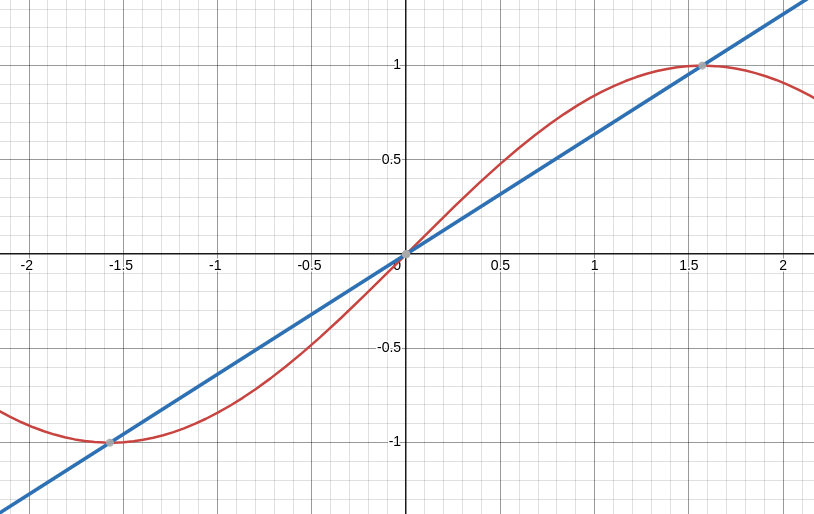
\includegraphics[width=6cm]{img/hw2/please}
  \caption{
    If $x$ is on the right half, $c$ is the left endpoint.
    If it's on the left, $c$ is the right endpoint.
    Either way, the line connecting $x$ and $c$ lies strictly above or below.
  }
\end{figure}

With that, let's $h_k$ just be $x-c$.
Since the intervals $x$ is in get smaller and smaller, $h_k$ should go to $0$ as well.

\subsubsection{Make Sure it Blows Up}

Now we somehow try to find that this monstrosity here:
\[\frac{\sum_{n=0}^{\infty} \frac{1}{2^n}\left(\sin\left(10^n(x+h_k)\right)-\sin\left(10^nx\right)\right)}{h_k}\]
diverges as $k \to \infty$.

We can split it in three parts.
For brevity, let $g_n(x)=\frac{\sin\left(10^n(x+h_k)\right)-\sin\left(10^nx\right)}{h_k}$:
\[\frac{g_k(x)}{2^k}+\sum_{n=0}^{k-1} \frac{g_n(x)}{2^n}+\sum_{n=k+1}^{\infty} \frac{g_n(x)}{2^n}\]
We've forced $g_k(x) \ge \frac{2 \cdot 10^k}{\pi}$,
so the first term is at least $\frac{2}{\pi} \cdot 5^k$.

Now we just need to make sure the other two summations don't screw us over.

\subsubsection{Please Work Oh My God}

$|\sin(x)-\sin(y)| \le 2$, so for the tail
\begin{align*}
  \left|\sum_{n=k+1}^{\infty} \frac{g_n(x)}{2^n}\right|
   & \le \sum_{n=k+1}^{\infty} \left|\frac{2}{2^n h_k}\right| \\
   & \le \left|\frac{1}{2^{k-1}h_k}\right|                    \\
   & \le \frac{4}{\pi} \cdot 5^k
\end{align*}

As for the first half, since $|\sin x - \sin y| \le |x-y|$,
\[\left|\sin\left(10^n(x+h_k)\right)-\sin\left(10^nx\right)\right| \le 10^nh_k\]
which bounds the head with
\[\sum_{n=0}^{k-1} \frac{g_n(x)}{2^n} \le \sum_{n=0}^{k-1} \frac{10^n}{2^n}=\frac{1}{4} \cdot 5^k - \frac{1}{4}\]

With these bounds, we have a bound that LITERALLY DOESN'T WORK IT'S SO COOKED
% \begin{align*}
%   \text{$k$th diff. quotient}
%    & = |\text{divergent} + \text{head} + \text{tail}|                                            \\
%    & \ge \frac{2}{\pi} \cdot 5^k - \frac{1}{\pi} \cdot 5^k - \frac{1}{4} \cdot 5^k - \frac{1}{4} \\
%    & \ge c \cdot 5^k - \frac{1}{4}
% \end{align*}
% for some $c > 0$, it doesn't really matter what it is.
% The point is that this is a divergent series as $k \to \infty$,
% so the limit can't exist.

\pagebreak

\section{Problem 3}

Lemme pull a stupid deus ex machina and write $g(x)=f(x)e^{-\lambda x}$.

Then, $g'(x)$ is
\[f(x)\left(-\lambda \cdot e^{-\lambda x}\right)+f'(x)e^{-\lambda x}=e^{-\lambda x}(-\lambda \cdot f(x)+f'(x))\]

Since $g(0)=g(1)=0$, there must be some $c \in (0, 1)$ at which $g'(c)=0$.

$e^{\lambda x} \ne 0$, so it must be $-\lambda \cdot f(c)+f'(c)$ that's $0$.

With some basic algebra, $-\lambda \cdot f(c)+f'(c)=0 \implies f'(c)=\lambda f(c)$. $\square$

\section{Problem 4}

\subsection{True if Not Max/Min}

Let $g(x)=f(x)-xf'(c)$.

It suffices to find $x_1, x_2 \in (0, 1)$ s.t. $g(x_1)=g(x_2)$ because then we have
\[f(x_1)-x_1f'(c)=f(x_2)-x_2f'(c) \implies f'(c)=\frac{f(x_1)-f(x_2)}{x_1-x_2}\]

BWOC say $g$ was injective.
Since it's also continuous, from class we know this means
$g$ is strictly monotonic.
WLOG assume it's strictly increasing, so by extension $g'$ is nonnegative.

However, $g'(x)=f'(x)-f'(c)$, and since $g'(c)=0$ isn't a max or a min,
$\exists c' \in (0, 1): g'(c') < g'(c)=0$, which is a contradiction.

If $g$ was strictly decreasing you could just swap the signs or
whatever and everything should still work out :trust: $\square$

\subsection{False if Max}

Consider the function $-\left(x-\frac{1}{2}\right)^3$
and its derivative $-3\left(x-\frac{1}{2}\right)^2$.

At $x=\frac{1}{2}$, $f'$ achieves its maximum value of $0$.

However, the equality given requires us to find two different values
$x_1, x_2 \in (0, 1)$ s.t. $f(x_1)-f(x_2)=0$.
However, as $f$ is injective, no such pair of numbers can exist.

\pagebreak

\section{Problem 5}

Let $h(x)=g(x)-f(x)$.

BWOC $\exists x_0, \epsilon > 0: h(x_0)=0$ and $h(x) > 0\ \forall x \in (x_0, x_0 + \epsilon)$.

$h'(x) \le F(g(x))-F(f(x))$, and at $f(x_0)=g(x_0)$ we know $h'(x_0) \le 0$.

Also, as the right neighborhood of $x$ is positive, $0 < d < \epsilon \implies \frac{h(x_0+d)}{d} > 0 \implies h'(x_0) \ge 0$.
This, combined with the above inequality, means $h'(x_0)=0$.

Now, for any $x \in (x_0, x_0 + \epsilon)$, since $g(x) > f(x)$,
\begin{align*}
  h'(x) & \le F(g(x))-F(f(x))   \\
        & \le |F(g(x))-F(f(x))| \\
        & \le L|g(x)-f(x)|      \\
        & = L \cdot h(x)
\end{align*}

Now, choose any $\delta_0$ so that $x_0 + \delta_0$ is in that above interval.
Since $h(x+\delta_0) > h(x_0)$,
the slope between these two points $m=\frac{h(x+\delta_0)-h(x_0)}{\delta_0}=\frac{h(x+\delta_0)}{\delta_0} > 0$.

Since $h'(x_0)=0$, the slope, difference quotient, whatever you wanna call it tends to $0$,
there has to be some smallest $0 < \delta_1 \le \delta_0$ s.t. $\frac{h(x+\delta_1)}{\delta_1}=m$.
Oh yeah, this thing does have to exist in the first place, and that's because $\delta_0$
itself also satisfies the conditions- we can always pick that if need be.

By the MVT, $\exists \delta_2 \in (0, \delta_1): h'(x+\delta_2)=\frac{h(x+\delta_1)}{\delta_1} = m$.
Notice that $(x + \delta_2, h(x + \delta_2))$ has to be below the line from point $(x_0, 0)$ to $(x_0+\delta_1, m \cdot \delta_1)$.
If it were above, its slope would be greater than $m$
and $\delta_1$ wouldn't be the smallest value satisfying its specified conditions.

Then, we have
\begin{align*}
  m & = h'(x_0+\delta_2)            \\
    & \le L \cdot h(x_0 + \delta_2) \\
    & \le L \cdot \delta_2 \cdot m
\end{align*}
which means $L \ge \frac{1}{\delta_2} > \frac{1}{\delta_1} \ge \frac{1}{\delta_0}$.

This is true for $\delta_0$ arbitrarily small, so no finite $L$ can exist, a contradiction. $\square$

\pagebreak

\section{Problem 6}

\subsection{Nonzero if Close}\label{sec:p6p1}

By Taylor's Theorem, for all $x \ne c$, $\exists x_1 \in (x, c)$ s.t.
\[g(x)=\sum_{k=0}^{n-1} \frac{g^{(k)}(c)}{k!}(x-c)^k + \frac{g^{(n)}(x_1)}{n!}(x-c)^n\]
The summation in this case is $0$ since $g^{(k)}=0$ for all $k$ from $0$ to $n-1$.
However, $g^{(n)}$ is nonzero everywhere, so $g(x)$ must be nonzero as long as $x \ne c$.

We can repeat the same argument for any $g^{(i)}$ where $0 \le i < n$, since we have
\[g^{(i)}(x)=\sum_{k=i}^{n-1} \frac{g^{(k)}(c)}{(k-i)!}(x-c)^{k-i} + \frac{g^{(n)}(x_1)}{(n-i)!}(x-c)^{n-i}\]
and the same things apply. $\square$

\subsection{Limits, Limits, Limits}

Since $f$ and $g$ both go to $0$ as $x \to c$ (as they're continuous),
\[\lim_{x \to c} \frac{f(x)}{g(x)}=\lim_{x \to c} \frac{f'(x)}{g'(x)}\]
As long as the limit on the RHS exists, the one on the left does too.
Since $f'(x)$ is only zero at $x=c$ as shown in \ref{sec:p6p1},
we'll never divide by $0$ within the limit.

As $\lim_{x \to c} g^{(i)}(x)=0$ for all $i$ from $0$ to $n-1$,
we can repeat LHopital's Rule to get
\[\lim_{x \to c} \frac{f(x)}{g(x)}
  =\lim_{x \to c} \frac{f^{(n-1)}(x)}{g^{(n-1)}(x)}\]

Now, $g^{(n)}(x) \ne 0$, so $\frac{f^{(n)}(x)}{g^{(n)}(x)} \in \R$ and
\begin{align*}
  \frac{f^{(n)}(x)}{g^{(n)}(x)}
  &= \frac{\lim_{x \to c} \frac{f^{(n-1)}(x)-f^{(n-1)}(c)}{x-c}}{\lim_{x \to c} \frac{g^{(n-1)}(x)-g^{(n-1)}(c)}{x-c}} \\
  &= \lim_{x \to c} \frac{\frac{f^{(n-1)}(x)-f^{(n-1)}(c)}{x-c}}{\frac{g^{(n-1)}(x)-g^{(n-1)}(c)}{x-c}} \\
  &= \lim_{x \to c} \frac{f^{(n-1)}(x)}{g^{(n-1)}(x)} \\
  &= \lim_{x \to c} \frac{f(x)}{g(x)}\quad\square
\end{align*}

\pagebreak

\section{Problem 7}

Fix $x$ and $y$ s.t. $x < y$.

By the MVT $\exists c_x \in (0, x): f'(c_x) = \frac{f(x)-f(0)}{x-0}=\frac{f(x)}{x}$.

We can also find by the same theorem a $c_y \in (x, y): f'(c_y) = \frac{f(y)-f(x)}{y-x}$.

$c_x \ge c_y$, so by the monotonicity of $f'$ we have
\begin{align*}
             & \frac{f(x)}{x} \le \frac{f(y)-f(x)}{y-x}                    \\
  \implies{} & f(x) \cdot y - f(x) \cdot x \le f(y) \cdot x - f(x) \cdot x \\
  \implies{} & f(x) \cdot y \le f(y) \cdot x                               \\
  \implies{} & \frac{f(x)}{x} \le \frac{f(y)}{y}\quad\square
\end{align*}

\pagebreak

\section{Problem 8}

Fix any $x$ and $d > 0$.

By Taylor's Theorem we have an $x_1 \in (x, x+2d)$ s.t.
\[f(x+2d)=f(x)+f'(x)((x+2d)-x)+\frac{f''(x)}{2}(x+2d-x)^2\]
Isolating $f'(x)$ gets us
\begin{align*}
  f'(x) & = \frac{f(x+2d)-f(x)-2d^2f''(x)}{2d}        \\
        & = \frac{1}{2d}(f(x+2d)-f(x))+d \cdot f''(x)
\end{align*}

Taking the absolute value of both sides gets us
\begin{align*}
  |f'(x)| & = \left|\frac{1}{2d}(f(x+2d)-f(x))+d \cdot f''(x)\right| \\
          & \le \frac{1}{2d}\left|f(x+2d)-f(x)\right| + d|f''(x)|    \\
          & \le \frac{1}{d}M_0 + dM_1
\end{align*}
and squaring both sides gets us
\[f'(x)^2 \le \frac{1}{d^2}M_0+d^2M_1^2+2M_0M_1\]

By AM-GM, $\frac{1}{d^2}M_0+d^2M_1^2 \le 2M_0M_1$, so we actually have
\[f'(x)^2 \le 4M_0M_1\]
for all $x$, which must mean $M_1^2 \le 4M_0M_1$. $\square$

\end{document}
